\documentclass[]{article}
\usepackage{lmodern}
\usepackage{amssymb,amsmath}
\usepackage{ifxetex,ifluatex}
\usepackage{fixltx2e} % provides \textsubscript
\ifnum 0\ifxetex 1\fi\ifluatex 1\fi=0 % if pdftex
  \usepackage[T1]{fontenc}
  \usepackage[utf8]{inputenc}
\else % if luatex or xelatex
  \ifxetex
    \usepackage{mathspec}
  \else
    \usepackage{fontspec}
  \fi
  \defaultfontfeatures{Ligatures=TeX,Scale=MatchLowercase}
\fi
% use upquote if available, for straight quotes in verbatim environments
\IfFileExists{upquote.sty}{\usepackage{upquote}}{}
% use microtype if available
\IfFileExists{microtype.sty}{%
\usepackage{microtype}
\UseMicrotypeSet[protrusion]{basicmath} % disable protrusion for tt fonts
}{}
\usepackage[margin=1in]{geometry}
\usepackage{hyperref}
\hypersetup{unicode=true,
            pdfborder={0 0 0},
            breaklinks=true}
\urlstyle{same}  % don't use monospace font for urls
\usepackage{color}
\usepackage{fancyvrb}
\newcommand{\VerbBar}{|}
\newcommand{\VERB}{\Verb[commandchars=\\\{\}]}
\DefineVerbatimEnvironment{Highlighting}{Verbatim}{commandchars=\\\{\}}
% Add ',fontsize=\small' for more characters per line
\usepackage{framed}
\definecolor{shadecolor}{RGB}{248,248,248}
\newenvironment{Shaded}{\begin{snugshade}}{\end{snugshade}}
\newcommand{\KeywordTok}[1]{\textcolor[rgb]{0.13,0.29,0.53}{\textbf{#1}}}
\newcommand{\DataTypeTok}[1]{\textcolor[rgb]{0.13,0.29,0.53}{#1}}
\newcommand{\DecValTok}[1]{\textcolor[rgb]{0.00,0.00,0.81}{#1}}
\newcommand{\BaseNTok}[1]{\textcolor[rgb]{0.00,0.00,0.81}{#1}}
\newcommand{\FloatTok}[1]{\textcolor[rgb]{0.00,0.00,0.81}{#1}}
\newcommand{\ConstantTok}[1]{\textcolor[rgb]{0.00,0.00,0.00}{#1}}
\newcommand{\CharTok}[1]{\textcolor[rgb]{0.31,0.60,0.02}{#1}}
\newcommand{\SpecialCharTok}[1]{\textcolor[rgb]{0.00,0.00,0.00}{#1}}
\newcommand{\StringTok}[1]{\textcolor[rgb]{0.31,0.60,0.02}{#1}}
\newcommand{\VerbatimStringTok}[1]{\textcolor[rgb]{0.31,0.60,0.02}{#1}}
\newcommand{\SpecialStringTok}[1]{\textcolor[rgb]{0.31,0.60,0.02}{#1}}
\newcommand{\ImportTok}[1]{#1}
\newcommand{\CommentTok}[1]{\textcolor[rgb]{0.56,0.35,0.01}{\textit{#1}}}
\newcommand{\DocumentationTok}[1]{\textcolor[rgb]{0.56,0.35,0.01}{\textbf{\textit{#1}}}}
\newcommand{\AnnotationTok}[1]{\textcolor[rgb]{0.56,0.35,0.01}{\textbf{\textit{#1}}}}
\newcommand{\CommentVarTok}[1]{\textcolor[rgb]{0.56,0.35,0.01}{\textbf{\textit{#1}}}}
\newcommand{\OtherTok}[1]{\textcolor[rgb]{0.56,0.35,0.01}{#1}}
\newcommand{\FunctionTok}[1]{\textcolor[rgb]{0.00,0.00,0.00}{#1}}
\newcommand{\VariableTok}[1]{\textcolor[rgb]{0.00,0.00,0.00}{#1}}
\newcommand{\ControlFlowTok}[1]{\textcolor[rgb]{0.13,0.29,0.53}{\textbf{#1}}}
\newcommand{\OperatorTok}[1]{\textcolor[rgb]{0.81,0.36,0.00}{\textbf{#1}}}
\newcommand{\BuiltInTok}[1]{#1}
\newcommand{\ExtensionTok}[1]{#1}
\newcommand{\PreprocessorTok}[1]{\textcolor[rgb]{0.56,0.35,0.01}{\textit{#1}}}
\newcommand{\AttributeTok}[1]{\textcolor[rgb]{0.77,0.63,0.00}{#1}}
\newcommand{\RegionMarkerTok}[1]{#1}
\newcommand{\InformationTok}[1]{\textcolor[rgb]{0.56,0.35,0.01}{\textbf{\textit{#1}}}}
\newcommand{\WarningTok}[1]{\textcolor[rgb]{0.56,0.35,0.01}{\textbf{\textit{#1}}}}
\newcommand{\AlertTok}[1]{\textcolor[rgb]{0.94,0.16,0.16}{#1}}
\newcommand{\ErrorTok}[1]{\textcolor[rgb]{0.64,0.00,0.00}{\textbf{#1}}}
\newcommand{\NormalTok}[1]{#1}
\usepackage{graphicx,grffile}
\makeatletter
\def\maxwidth{\ifdim\Gin@nat@width>\linewidth\linewidth\else\Gin@nat@width\fi}
\def\maxheight{\ifdim\Gin@nat@height>\textheight\textheight\else\Gin@nat@height\fi}
\makeatother
% Scale images if necessary, so that they will not overflow the page
% margins by default, and it is still possible to overwrite the defaults
% using explicit options in \includegraphics[width, height, ...]{}
\setkeys{Gin}{width=\maxwidth,height=\maxheight,keepaspectratio}
\IfFileExists{parskip.sty}{%
\usepackage{parskip}
}{% else
\setlength{\parindent}{0pt}
\setlength{\parskip}{6pt plus 2pt minus 1pt}
}
\setlength{\emergencystretch}{3em}  % prevent overfull lines
\providecommand{\tightlist}{%
  \setlength{\itemsep}{0pt}\setlength{\parskip}{0pt}}
\setcounter{secnumdepth}{0}
% Redefines (sub)paragraphs to behave more like sections
\ifx\paragraph\undefined\else
\let\oldparagraph\paragraph
\renewcommand{\paragraph}[1]{\oldparagraph{#1}\mbox{}}
\fi
\ifx\subparagraph\undefined\else
\let\oldsubparagraph\subparagraph
\renewcommand{\subparagraph}[1]{\oldsubparagraph{#1}\mbox{}}
\fi

%%% Use protect on footnotes to avoid problems with footnotes in titles
\let\rmarkdownfootnote\footnote%
\def\footnote{\protect\rmarkdownfootnote}

%%% Change title format to be more compact
\usepackage{titling}

% Create subtitle command for use in maketitle
\newcommand{\subtitle}[1]{
  \posttitle{
    \begin{center}\large#1\end{center}
    }
}

\setlength{\droptitle}{-2em}

  \title{}
    \pretitle{\vspace{\droptitle}}
  \posttitle{}
    \author{}
    \preauthor{}\postauthor{}
    \date{}
    \predate{}\postdate{}
  

\begin{document}

\doublespacing

\textbf{\section{Introduction}} \label{sec3:Introduction}

The fundamental premise in the nature behind ORMFs, is to provide an
exposure-based treatment of OpRisk losses which caters to modeling
capital estimates for forward-looking aspects of ORM. This proves tricky
due to the lag between the time the loss event occurs and the actual
realised loss, i.e.~by the very nature of OpRisk, there is a significant
lag between the moment the OpRisk event is conceived to the moment the
event is observed and accounted for. There is a gap in time between
\(\tau\) the moment the risk is conceived and the time \(\tau+1\) when
impact of the loss is realised. This timing paradox often results in
questionable capital estimates, especially for those near misses,
pending and realised losses that need to be captured in the model

\section{EBOR methodology for capturing forward-looking aspects of ORM}
\label{sec:EBOR methodology for capturing forward-looking aspects of ORM}

@einemann2018operational, in a theoretical paper, construct a
mathematical framework for an EBOR model to quantify OpRisk for a
portfolio of pending litigations. Their work unearths an invaluable
contribution to the literature, discussing a strategy on how to
integrate EBOR and LDA models by building hybrid frameworks which
facilitate the migration of OpRisk types from a \emph{classical} to an
exposure-based treatment through a quantitative framework, capturing
forward looking aspects of BEICF's {[}@einemann2018operational{]}, a key
source of the OpRisk data.

The measure of exposure we need to use depends specifically on
projecting the number of OpRisk event types (frequency of losses) as the
target variable in the model and is different to the measure if the
target variable were the severity of the losses. As per definition
\ref{ssec:Definition of exposure}, the lag represents exposure; we need
historical exposure for experience rating because we need to be able to
compare the loss experience of different years on a like-for-like basis
and to adjust it to current exposure levels
{[}@parodi2014pricing{]}.\medskip 

With reference to the current section, Section
\ref{sec:EBOR methodology for capturing forward-looking aspects of ORM},
the fundamental premise behind the LDA is that each firm's OpRisk losses
are a reflection of it's underlying Oprisk exposure. In particular, the
assumption behind the use of the Poisson distribution in the model to
estimate the frequency of losses, is that both the the intensity (or
rate) of occurrence and the opportunity (or exposure) for counting are
constant for all available observations.\medskip

\subsection{Limitations of the EBOR model}

In their model {[}@einemann2018operational{]}, the definition of
exposure, Definition \ref{ssec:Definition of exposure}, is particularly
well-suited to the specific risk type dealt with in their paper i.e.,
the portfolio of litigation events, due to better usage of existing
information and more plausible model behavior over the litigation life
cycle. However, it is bound to under-perform for many other OpRisk event
types since these EBOR models are typically designed to quantify
specific aspects of OpRisk i.e., litigation risk have rather
concentrated risk profiles. Furthermore, EBOR models are important due
to wide applicability beyond capital calculation and its potential to
evolve into an important tool for auditing process and early detection
of potential losses.

\textbf{\section{Generalised Linear Models (GLM's)}}
\label{sec:Generalised Linear Models}

Operational riskiness in FIs grows as trading transactions grow in
complexity, i.e.~the more complex and numerous trading activity builds
the higher the rate at which new cases of OpRisk events occur.
Therefore, it is likely that the rate of operational hazard may be
increasing exponentially over time. The scientifically interesting
question is whether the data provides any evidence that the increase in
the underlying operational hazard generation is slowing.\medskip

By the aforementioned postulate from the obove paragraph provides a
plausible model to start investigating this question. The model assumes
that if \(\mu_i\) is the (rate) number of expected new OpRisk events per
time interval \(\tau - \tau+1 = \tau_i\) since the beggining of the
data, then \(\mu_i\) increases according to: \singlespacing

\begin{eqnarray}
\mu_i = \gamma \mbox{exp}({\delta\tau_i}) \nonumber
\end{eqnarray}

\doublespacing

where \(\gamma\) and \(\delta\) are unknown parameters. Taking a log
link turns the model into Generalised Linear Model (GLM) form so that:

\singlespacing

\begin{eqnarray}\label{eqn:simplepoisson}
\mbox{log}(\mu_i) = \mbox{log}(\gamma) + \delta\tau_i = \beta_0 + \tau_i\beta_1
\end{eqnarray}

\doublespacing

Where the LHS is

\begin{math} y_i \sim \mbox{Poi}(\mu_i) \end{math}

is the observed number of new cases over time \(\tau\) and \(\tau+1\),
and the RHS is a linear in the parameters
\(\beta_0 = \mbox{log}(\gamma)\) and \(\beta_1 = \delta\).\medskip

We define a binary variable LossIndicator, which takes on a value \(1\)
for realised losses and a value \(0\) for pending losses, and/or near
misses, showing the number of relevant Oprisk event's incidence in a
specified time interval \(\tau\) and \(\tau+1\). A quadratic term
(\(\beta_2t_i^2\)) could be added to the model so that its residual
values increase monotonically with time as the fitted values do, which
usefully approximates other situations which may influence the counts
adapted to the poisson case.

\singlespacing

\begin{eqnarray}\label{eqn:adaptedpoisson}
\mu = d_i\mbox{exp}(\beta_0 + \beta_1\tau_i + \beta_2{\tau_i}^2) 
\end{eqnarray}

\doublespacing

\subsection{GLM for count data}

The LHS of a GLM formula is the model's random component i.e.,
observations of the number of OpRisk transactions over the trading
transaction period in an FI's portfolio; given by the independent random
variables \(y_1, y_2,\ldots, y_n\), not i.i.d {[}@wood2017generalized,
@covrig2015using{]}. \(Y\) takes a (exponential) family argument,
depending on parameters \(ln\lambda\), where \(\lambda\) which
represents the average frequency of the OpRisk transactions. It is worth
distinguishing between the response data \(y_i\) which is an observation
of \(Y\).\medskip

\textbf{\section{A poisson regression operational hazard model}}
\label{sec:A poisson regression operational hazard model}

The target variable (LossIndicator) which shows the number of relevant
Oprisk event's incidence in a specified time interval \(\tau\) and
\(\tau+1\) is count data, justifying the choice of poisson distribution
a reasonable model. It's probability mass function (pdf) is:

\singlespacing

\begin{eqnarray}\label{eqn:Poisson}
Y &\sim& \mbox{poisson}(\lambda), \quad f(y;\lambda) = \frac{\lambda^y}{y!}\dot\exp{-y}\\
 &\mbox{where}& \quad y \in  \mathbb{N}, \mbox{and} \quad \lambda > 0 \nonumber
\end{eqnarray}

\doublespacing

the expectation and variance
\(E[Y] = \mbox{VaR}[Y] = \lambda\)\footnote{If you were to guess an independent $Y_i$ from a random sample, the best guess is given by this expression},
are both equal to parameter \(\lambda\) simultaneously. The RHS of
Equation \ref{eqn:Poisson} is the model's systematic component, and it
specifies the linear predictor. It builds on equation
\ref{eqn:adaptedpoisson} with \(p+1\) parameters,
\(\beta = (\beta_0\ldots,\beta_p)^t\), and \(p\) explanatory variables:

\singlespacing

\begin{eqnarray}
\nu = \beta_0 + \sum_{j=1}^{p}\beta_jx_{ij}, \qquad \mbox{where} \quad i = 1,\ldots,n
\end{eqnarray}

\doublespacing

If sample variables \(Y_i \sim \mbox{Poisson}(\lambda_i)\), then
\(\mu = E[Y_i] = \lambda_i\); the link function between the random and
systematic components, viz. a tranformation by the model by some
function \(g()\), which does not change features essential to to
fitting, but rather a scaling in magnitude so that:

\singlespacing

\begin{eqnarray}\label{eqn:linkfcn }
\nu_i &=& g(\lambda_i) = \mbox{ln}\lambda_i, \qquad \mbox{that is} \nonumber \\
\nu &=& \beta_0 + \sum_{j=1}^{p}\beta_jx_{ij}
\end{eqnarray}

\doublespacing

so the mean frequency or otherwise the rate \(R\), will be predicted by
the model\ldots

\singlespacing

\begin{eqnarray}\label{eqn:multmodel}
\lambda_i &=& d_i\mbox{exp}(\beta_0 + \sum_{j=1}^{p}\beta_jx_{ij}) \quad \mbox{or} \nonumber \\
\lambda_i &=& d_i\cdot e^{\beta_0}\cdot e^{\beta_1x_{i1}}\cdot e^{\beta_2x_{i2}} \ldots e^{\beta_px_{ip}}
\end{eqnarray}

\doublespacing

Where \(d_i\) represents the risk exposure for transaction \(i\). Taking
logs on both sides of equation \ref{eqn:multmodel}, the regression model
for the estimation of loss frequency is:

\singlespacing

\begin{eqnarray}
\mbox{ln}\lambda_i =  \mbox{ln}d_i + \beta_0 + \beta_1x_{i1} + \beta_2x_{i2} + \ldots + \beta_px_{ip}
\end{eqnarray}

\doublespacing

where \(\mbox{ln}d_i\) is the natural log of risk exposure, called the
``offset variable''.

\subsection{Interpretation}

Table \ref{tab_int} presents the various units produced for the various
GLM links.

\begin{Shaded}
\begin{Highlighting}[]
\NormalTok{tab <-}\StringTok{ }\KeywordTok{data.frame}\NormalTok{(}\StringTok{"Link Function"}\NormalTok{=}\KeywordTok{c}\NormalTok{(}\StringTok{"Identity"}\NormalTok{, }\StringTok{"Log"}\NormalTok{, }\StringTok{"Logit"}\NormalTok{, }\StringTok{"Probit"}\NormalTok{, }\StringTok{"Poisson"}\NormalTok{, }\StringTok{"Gamma"}\NormalTok{, }\StringTok{"Negative Binomial"}\NormalTok{),}
                  \StringTok{"Average Marginal Effect"}\NormalTok{=}\KeywordTok{c}\NormalTok{(}\StringTok{"Original Continuous Unit"}\NormalTok{, }\StringTok{"Original Continuous Unit"}\NormalTok{, }\StringTok{"Risk"}\NormalTok{, }\StringTok{"Risk"}\NormalTok{, }\StringTok{"Count"}\NormalTok{, }\StringTok{"Count"}\NormalTok{, }\StringTok{"Count"}\NormalTok{))}
\KeywordTok{names}\NormalTok{(tab) =}\StringTok{ }\KeywordTok{c}\NormalTok{(}\StringTok{"Link Function"}\NormalTok{, }\StringTok{"Average Marginal Effect"}\NormalTok{)}
\KeywordTok{options}\NormalTok{(}\DataTypeTok{xtable.comment =} \OtherTok{FALSE}\NormalTok{)}
\KeywordTok{library}\NormalTok{(xtable)}
\NormalTok{tabx =}\StringTok{ }\KeywordTok{xtable}\NormalTok{(tab, }
       \DataTypeTok{label =} \StringTok{"tab_int"}\NormalTok{, }
       \DataTypeTok{caption =} \StringTok{"The generalized linear model link functions with their associated units of interpretation. Note: This list is not exhaustive and there are likely more GLMs that are used within prevention research."}\NormalTok{,}
       \DataTypeTok{align =} \KeywordTok{c}\NormalTok{(}\StringTok{"l"}\NormalTok{, }\StringTok{"|l"}\NormalTok{, }\StringTok{"|c|"}\NormalTok{))}
\KeywordTok{print.xtable}\NormalTok{(tabx, }\DataTypeTok{include.rownames =} \OtherTok{FALSE}\NormalTok{, }\DataTypeTok{caption.placement =} \StringTok{"top"}\NormalTok{,}
             \DataTypeTok{table.placement =} \StringTok{"tb"}\NormalTok{)}
\end{Highlighting}
\end{Shaded}

\begin{table}[tb]
\centering
\caption{The generalized linear model link functions with their associated units of interpretation.} 
\label{tab_int}
\begin{tabular}{lc}
\toprule
Link Function & Target variable Effect \\ 
\midrule
Identity & Original Continuous Unit \\ 
  Log & Original Continuous Unit \\ 
  Logit & Risk \\ 
  Probit & Risk \\ 
  Poisson & Count \\ 
  Gamma & Count \\ 
  Negative Binomial & Count \\ 
\bottomrule
\end{tabular}
\end{table}

The poisson distribution is restrictive when applied to approximate
counts, due to the assumption made about it that the mean and variance
of the number of events are equal. However, in models for count data
where means are low so that the number of zeros and ones in the data is
exessive are well adapted to the poisson case
{[}@wood2017generalized{]}. These cases are characteristic of scenarios
in OpRisk other than those modeling situations when the unchecked
spreading of negligent behaviour may result in an operational hazard.
For example, the negative binomial and/or quasipoisson regression models
ascribe to data that exhibits \emph{overdispersion}, wherein the
variance is much larger than the mean for basic count data, therefore
they have been eliminated in this paper.

\textbf{\section{Research Objective 1}} \label{sec:Research Objective 1}

To introduce the generalised additive model for location, scale and
shape (GAMLSS) framework for OpRisk management, that captures exposures
to forward-looking aspects in the OpRisk loss prediction problem, due to
deep hierarchies in the features of covariates in the investment banking
(IB) business environment, and internal control risk factors (BEICF)
thereof.

\textbf{\section{Exploratory data analysis}}

The main source of the analysis dataset is primary data, a collection of
internal OpRisk losses for the period between 1 January 2013 and 31st
March 2013 at an investment bank in SA. The method of data generation
and collection is at the level of the individual trade deal, wherein
deal information is drawn directly from the trade generation and and
settlement system (TGSS) and edit detail from attribution reports
generated in middle office profit \& loss (MOPL). The raw source
consists of two separate datasets on a trade-by-trade basis of daily
frequencies (number of events) and associated loss severities.\medskip

The raw frequency data consists of 58,953 observations of 15 variables,
within the dataset there are 50,437 unique trades. The raw severity data
consists of 6,766 observations of 20 variables; within the severity
dataset there are 2,537 unique trades. The intersection between the
frequency and severity datasets consists of 2,330 individual
transactions which represent realised losses, pending and/or near
misses. This dataset is comprised of 3-month risk correction detail, in
the interval between 01 January 2013 and 31 March 2013. \medskip

\begin{verbatim}
## Warning: package 'rattle' was built under R version 3.5.3
\end{verbatim}

\begin{verbatim}
## Rattle: A free graphical interface for data science with R.
## Version 5.2.0 Copyright (c) 2006-2018 Togaware Pty Ltd.
## Type 'rattle()' to shake, rattle, and roll your data.
\end{verbatim}

\begin{verbatim}
## 
## Attaching package: 'Hmisc'
\end{verbatim}

\begin{verbatim}
## The following objects are masked from 'package:xtable':
## 
##     label, label<-
\end{verbatim}

\begin{verbatim}
## The following objects are masked from 'package:base':
## 
##     format.pval, units
\end{verbatim}

\begin{verbatim}
## 
## Attaching package: 'dplyr'
\end{verbatim}

\begin{verbatim}
## The following objects are masked from 'package:Hmisc':
## 
##     src, summarize
\end{verbatim}

\begin{verbatim}
## The following objects are masked from 'package:stats':
## 
##     filter, lag
\end{verbatim}

\begin{verbatim}
## The following objects are masked from 'package:base':
## 
##     intersect, setdiff, setequal, union
\end{verbatim}

\begin{table}[ht]
\centering
\caption{The contents of the traded transactions of the associated risk correction events.}
\begin{tabular}{lcc}
\toprule
  & \multicolumn{2}{c}{Storage} \\
Covariate     & Levels   & Type \\ 
\midrule
 Trade       &          & numeric \\
 UpdateTime  &          & numeric \\
 UpdatedDay  &          & numeric \\
 UpdatedTime &          & numeric \\
 TradeTime   &          & numeric \\
 TradedDay   &          & numeric \\
 TradedTime  &          & numeric \\
 Desk        &  10      & categorical \\
 CapturedBy  &  5       & categorical \\
 TradeStatus &  4       & categorical \\
 TraderId    &  7       & categorical \\
 Instrument  &  23      & categorical \\
 Reason      &  19      & categorical \\
 Loss        &          & numeric \\
 EventTypeCategoryLevel & 5  & categorical \\
 BusinessLineLevel      & 8  & categorical \\
 LossIndicator          & 2  & binary \\
 exposure               &    & numeric \\
 \bottomrule
\end{tabular}\label{tab_contents}
\end{table}

Two new variables are derived from the data; a target variable
(LossIndicator) is a binary variable whereupon, a \(1\) signifies a
realised loss, and \(0\) for those pending losses, or near misses. The
\emph{exposure} variable is computed by deducting the time between the
trade amendment (UpdateTime) and the time when the trade was booked
(TradeTime). It is a measure that is meant to be rougly proportional to
the risk of the transaction or a group of transactions. The idea is that
if the exposure (e.g.~the duration of a trade, the number of
allocation(trade splits), etc.) doubles whilst everything else (e.g.~the
rate, nominal of the splits, and others) remains the same, then the risk
also doubles.

In R, the GLM function works with two types of covariates/explanatory
variables: numeric (continuous) and categorical (factor) variables as
depicted in table \ref{tab_contents}. Multi-level categorical variables
are recoded by building dummy variables corresponding to each level.
This is achieved through an implemented algorithm in R, through a
transformation as recommended for the estimation of the GLM,
particularly in the estimation of the poisson regression model for count
data.

The model revolves around the fact that for each categorical variable
(covariate), previously transformed into a dummy variable, one must
specify a reference category from which the corresponding observations
under the same covariate are estimated and assigned a weight against in
the model {[}@covrig2015using{]}. By default in the GLM, the first level
of the categorical variable is taken as the reference level. As best
practice, @de2008generalized, @frees2010household, @denuit2007actuarial,
@cameron2013regression and others recommend that for each categorical
variable one should specify the modal class as the reference level; as
this variable corresponds to the level with the highes order of
predictability, excluding the dummy variable corrresponding to (weight
coefficient = \(0\)) the biggest absolute frequency.

\textbf{\section{Description of the dataset}}
\label{sec:Description of the dataset}

In this section, section \ref{sec:Description of the dataset}, the
dataset called \emph{OpRiskDataSet\_exposure}, provides data on the
increase in the numbers of operational events over a three month period,
beginning 01 January 2013 to end of 20 March 2013. For each transaction,
there is information about: trading risk exposure, trading
characteristics, causal factor characteristics and their cost.

\begin{figure}
\begin{subfigure}[b]{0.55\textwidth}
   \begin{frame}
      \centering
       \begin{tabular}{cc}
        \textbf{Intra-day Trend of Loss Severity} & \textbf{Trends of Loss Severities per Trader} \\
        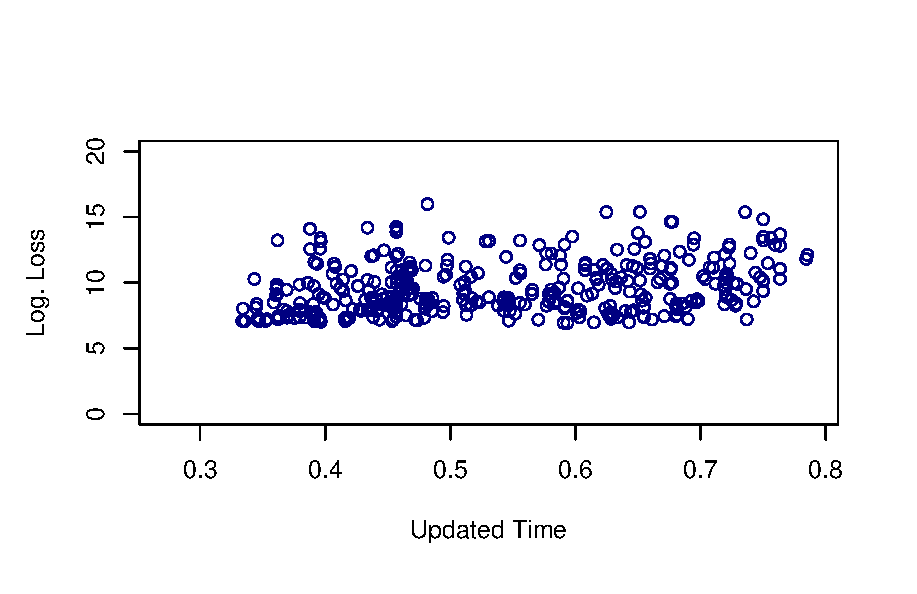
\includegraphics[width=7.5cm]{IntraDayUpdatedTime.eps}
         &
         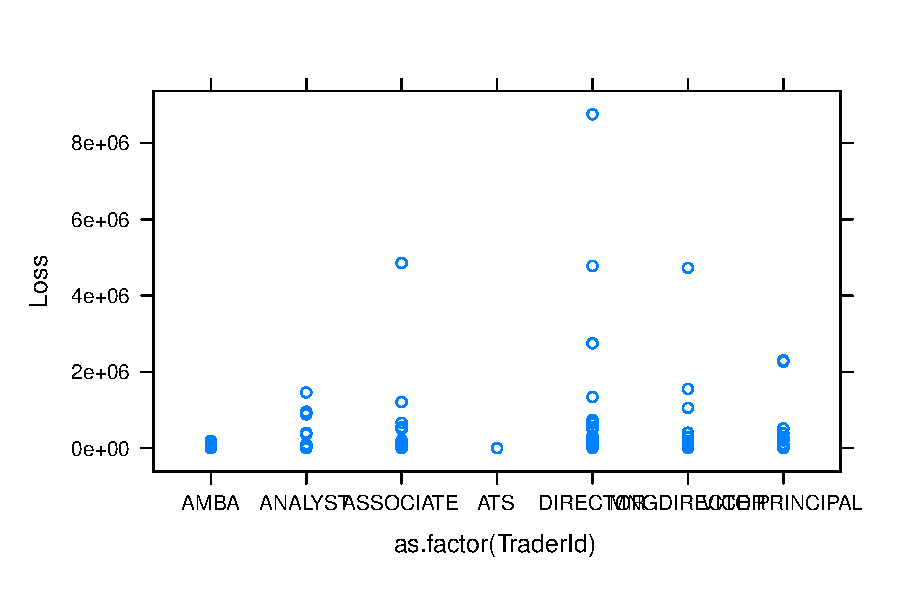
\includegraphics[width=7cm]{TrendTraderId.eps}
         \end{tabular}
    \end{frame}
\subcaption{Scatterplots}
   \label{Intra_Day_Trends} 
\end{subfigure}

\begin{subfigure}[b]{0.55\textwidth}
   \begin{frame}
      \centering
       \begin{tabular}{cc}
        \textbf{Loss per month} & \textbf{Trading frequency} \\
        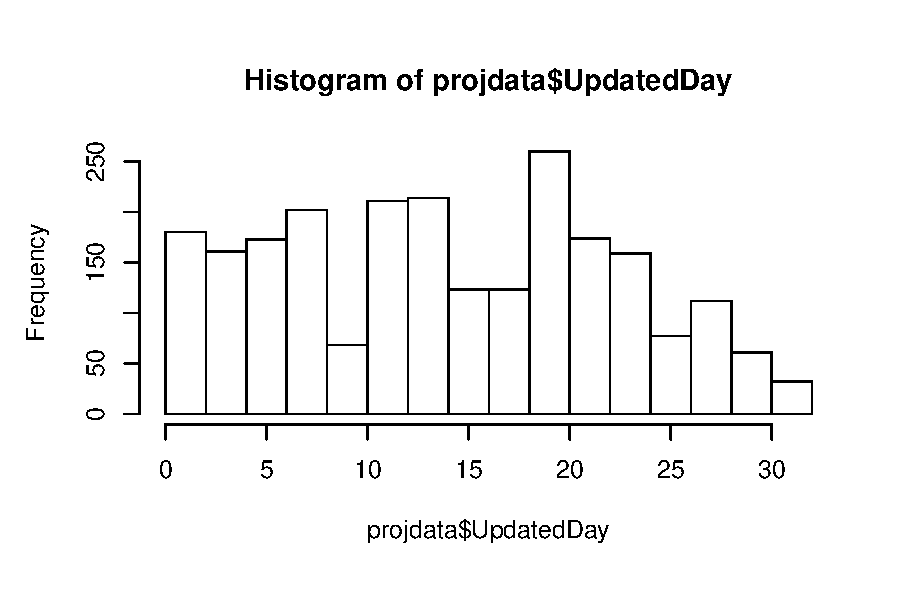
\includegraphics[width=7.5cm]{UpdatedDayFreq.eps}
         &
         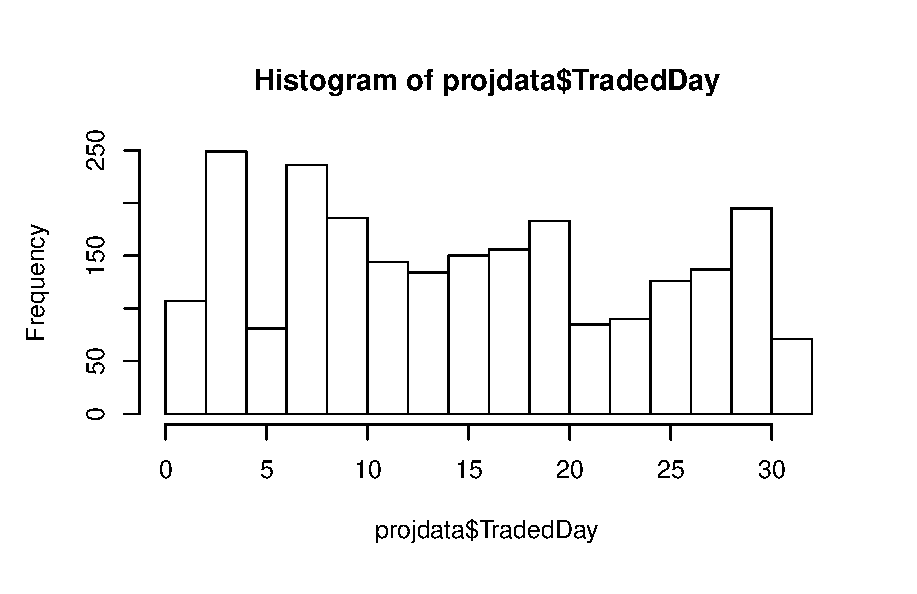
\includegraphics[width=7cm]{TradedDayFreq.eps}
         \end{tabular}
    \end{frame}
\subcaption{Histograms}
   \label{Hist_Loss_Freq}
\end{subfigure}
\caption[Numerical grid display]{(a) Scatterplots of intra-day trend analysis for logs of severities of operational events and trends incident activity for identifying the role of the trader originating the incidents. (b) As for (a) but in the form of histograms showing the frequency distrbution of the number daily operational indicents and the number of trades over a monthly period.} 
\end{figure}

\subsection{Characteristics of exposure}

The exposure of risk of type \(i\), \(d_i\) shows the daily duration,
from when the trade was booked to the moment the operational risk event
was observed and ended. This measure is defined this way when
specifically applied to projecting the number of loss events
(frequencies) and can be plotted as follows depicted in graphs depicted
in Figure \ref{Exploration_analysis_exposure}.\medskip

\begin{verbatim}
## 
## Attaching package: 'reshape'
\end{verbatim}

\begin{verbatim}
## The following object is masked from 'package:dplyr':
## 
##     rename
\end{verbatim}

\begin{figure}
\begin{frame}
      \centering
       \begin{tabular}{ccc}
        \textbf{Distribution} & \textbf{Density} & \textbf{Digital Analysis} \\
        \includegraphics[width=5cm]{Exposure_cdf.eps}
         &
         \includegraphics[width=5cm]{Dist_exposure.eps}
         &
         \includegraphics[width=5cm]{Benford.eps}
         \end{tabular}
    \end{frame}
        \captionof{figure}{A simple comparison of the Sigmoidal like features of the fat-tailed, right skewed distribution for exposure, and first-digit frequency distribution from the exposure data with the expected distribution according to Benford's Law}
    \label{Exploration_analysis_exposure}
\end{figure}

The variable follows a logistic trend on \([0,1]\), implying an FIs
operational risk portfolio rises like a sigmoid function throughout the
period of observation, typically starting from \(0\), which then
observes a plateau in growth. The average exposure is 389.99 or about 1
year.\medskip

Grid plots \ref{Exploration_analysis_exposure} portray the logistic
function, together with a simple comparison of first-digit frequency
distribution analysis, according to Benford's Law, with exposure data
distribution. The close fitting nature implies the data are uniformly
distributed across several orders of magnitude, especially within the 1
year period.\medskip

\subsection{Characteristics of the covariates}

The characteristics of the operational risk portfolio are given by the
following covariates: \emph{UpdatedDay}, \emph{UpdatedTime} - the day of
the month and time of day the OpRisk incident occurs respectively;
\emph{TradedDay}, \emph{TradedTime} - the day in the month and time of
day the deal was originated respectively; The \emph{LossIndicator} as
indicated before is a binary variable consisting of two values: A \(0\),
which indicates pending or near misses, and \(1\), if the incident
results in a realised loss, meaning that there is significant p\&L
impact due to the OpRisk incident.\medskip

the \emph{Desk} is the location in the portfolio tree the incident
originated, it is a factor variable conisting of 10 categories;
\emph{CapturedBy}, the designated analyst who actions the incident, a
factor variable consisting of 5 categories; \emph{TraderId}, the trader
who originates the deal, a factor variable with 7 categories;
\emph{TradeStatus}, the live status of the deal, a factor variable with
4 categories; \emph{Instrument}, the type of deal, a factor variable
with 23 categories; \emph{Reason}, a description of the cause of the
OpRisk incident, a factor variable with 19 levels;
\emph{EventTypeCategoryLevel}, 7 OpRisk event types as per
@risk2001supporting, a factor variable with 5 categories;
\emph{BusinessLineLevel}, 8 OpRisk business lines as per
@risk2001supporting, a factor variable with 8 categories.\medskip

The factor variables were transformed into dummy variables using the
following commands: \singlespacing

\begin{Shaded}
\begin{Highlighting}[]
\CommentTok{# Remap factor variables and transform into numeric variables.}
\NormalTok{crs}\OperatorTok{$}\NormalTok{dataset[[}\StringTok{"TNM_Desk"}\NormalTok{]] <-}\StringTok{ }\KeywordTok{as.numeric}\NormalTok{(crs}\OperatorTok{$}\NormalTok{dataset[[}\StringTok{"Desk"}\NormalTok{]])}
\NormalTok{crs}\OperatorTok{$}\NormalTok{dataset[[}\StringTok{"TNM_CapturedBy"}\NormalTok{]] <-}\StringTok{ }\KeywordTok{as.numeric}\NormalTok{(crs}\OperatorTok{$}\NormalTok{dataset}
\NormalTok{                                              [[}\StringTok{"CapturedBy"}\NormalTok{]])}
\NormalTok{crs}\OperatorTok{$}\NormalTok{dataset[[}\StringTok{"TNM_TraderId"}\NormalTok{]] <-}\StringTok{ }\KeywordTok{as.numeric}\NormalTok{(crs}\OperatorTok{$}\NormalTok{dataset[[}\StringTok{"TraderId"}\NormalTok{]])}
\NormalTok{crs}\OperatorTok{$}\NormalTok{dataset[[}\StringTok{"TNM_Instrument"}\NormalTok{]] <-}\StringTok{ }\KeywordTok{as.numeric}\NormalTok{(crs}\OperatorTok{$}\NormalTok{dataset}
\NormalTok{                                              [[}\StringTok{"Instrument"}\NormalTok{]])}
\NormalTok{crs}\OperatorTok{$}\NormalTok{dataset[[}\StringTok{"TNM_Reason"}\NormalTok{]] <-}\StringTok{ }\KeywordTok{as.numeric}\NormalTok{(crs}\OperatorTok{$}\NormalTok{dataset[[}\StringTok{"Reason"}\NormalTok{]])}
\NormalTok{crs}\OperatorTok{$}\NormalTok{dataset[[}\StringTok{"TNM_EventTypeCategoryLevel1"}\NormalTok{]] <-}\StringTok{ }\KeywordTok{as.numeric}\NormalTok{(crs}\OperatorTok{$}\NormalTok{dataset}
\NormalTok{                                        [[}\StringTok{"EventTypeCategoryLevel1"}\NormalTok{]])}
\NormalTok{crs}\OperatorTok{$}\NormalTok{dataset[[}\StringTok{"TNM_BusinessLineLevel1"}\NormalTok{]] <-}\StringTok{ }\KeywordTok{as.numeric}\NormalTok{(crs}\OperatorTok{$}\NormalTok{dataset}
\NormalTok{                                             [[}\StringTok{"BusinessLineLevel1"}\NormalTok{]])}
\end{Highlighting}
\end{Shaded}

\doublespacing

The continuous numerical variable \emph{Loss}, shows the financial
impact (severity) of the OpRisk incident in Rands. For the most part
(i.e.~96.1\% of the time) OpRisk incidents result in pending losses
and/or near misses, most realised losses (2.3\%) lie within the
{[}\textbf{R$200,00$}, \textbf{R$300,000$}{]} range. In the current
portfolio there are also five p\&L impacts higher than
\textbf{R$2.5$ million}.\medskip

\subsection{Characteristics of daily operational activity}

The distribution of daily losses and/or pending/near misses by
operational activities are represented in
\ref{Exploratory_Time_Day_Frequency3plot}. Figure
\ref{Exploratory_UpdateTime_Frequency3plot} shows that most operational
events occur in times leading up to midday (i.e.~10:50AM to 11:50AM),
the observed median is 11:39AM, and of these potential loss events, most
realised losses occur closest to mid-day. The frequencies of the loss
incidents in the analysed portfolio sharply decreases during the
following period, i.e.~from 12:10PM to 13:10PM, during which the least
realised losses occur.\medskip

Figure \ref{Exploratory_UpdateDay_Frequency3plot} shows that operational
activity increases in intensity in the days leading up to the middle of
the month, i.e. \(10^{th}\) - \(15^{th}\); the observed mean is
\(14.49\) days, and of these potential loss events, realised losses
especially impact on the portfolio during these days.

\singlespacing

\doublespacing

\begin{figure}
\centering
\begin{subfigure}[b]{0.55\textwidth}
   \includegraphics[width=1\linewidth]{Exploratory_UpdateTime_Frequency3plot.eps}
   \subcaption{Frequency distributions of operational incidents by the time in the day}
   \label{Exploratory_UpdateTime_Frequency3plot} 
\end{subfigure}

\begin{subfigure}[b]{0.55\textwidth}
   \includegraphics[width=1\linewidth]{Exploratory_UpdateDay_Frequency3plot.eps}
   \subcaption{Frequency distributions of operational incidents by the day in the month}
   \label{Exploratory_UpdateDay_Frequency3plot}
\end{subfigure}

\caption[Two numerical solutions: Histograms showing the distribution of UpdatedTime \& UpdatedDay by LossIndicator.]{The frequency distributions of All the losses, the realised losses, and pending/near misses of operational incidents by the day in the month when the indidents' occurred}
\label{Exploratory_Time_Day_Frequency3plot}
\end{figure}

Similarly, the influence of trading desk's on the frequency of
operational events can be analysed on the basis of the portfolio's
bidimensional distribution by variables \emph{Desk} and
\emph{LossIndicator}, which shows the proportions realised losses vs
pending and/or near misses for each particular desk. The bidimensional
distribution of \emph{Desk} and \emph{LossIndicator} is presented in a
contingency table, Table \ref{tab_Desk_Prop}, in which it's considered
useful to calculate proportions for each desk category.

\begin{figure}
\centering
\includegraphics[width=20cm,height=5cm]{Density_UpdateDay_TradedDay.eps}
\caption[Density plots showing a comparison of realised vs pending losses and/near misses over a month for the day in the month the OpRisk incident was updated to the day in the month trades were traded/booked]{Density plots showing a comparison of realised vs pending losses and/near misses over a month for the day in the month the OpRisk incident was updated to the day in the month trades were traded/booked}
\label{Desk_Proportions}
\end{figure}

\singlespacing

\doublespacing

\begin{table}[ht]
\centering
\caption{Occurence of realised losses: proportions on desk categories}
\begin{tabular}{lccr}
\toprule
  & \multicolumn{3}{c}{No. of transactions} \\
Desk   & no Loss   & Loss & Total\\ 
\midrule
  Africa            &  49 & 10 &  59 \\
  Bonds/Repos       & 113 & 31 & 144 \\
  Commodities       & 282 & 45 & 327 \\
  Derivatives       & 205 & 24 & 229 \\
  Equity            & 269 & 66 & 335 \\
  Management/Other  &  41 &  2 &  43 \\
  Money Market      & 169 & 52 & 221 \\
  Prime Services    & 220 & 62 & 282 \\
  Rates             & 336 & 53 & 389 \\
  Structured Notes  & 275 & 26 & 301 \\
 \bottomrule
\end{tabular}\label{tab_Desk_Prop}
\end{table}

Thus, as illustratred in figure \ref{Desk_Proportions}, from 23,5\%; the
highest proportion of realised losses per desk is the Money Market (MM)
desk, the figures are decreasing, followed by Prime Services (22\%);
Bonds/Repos (21,5\%); Equity (19,7\%); Africa (16,9\%); Commodities
(13,8\%); Rates (13,6\%); Derivatives (10,5\%); Structured Notes (SND)
(8.6\%), to the least proportion in the Management/Other, a category
where only 4,7\% of operations activities were realised as losses.

\singlespacing

\begin{verbatim}
## Joining, by = "Desk"
\end{verbatim}

\doublespacing

\begin{figure}
\centering
\includegraphics[width=20cm,height=5cm]{Exploratory_Desk_Proportions.eps}
\caption[Desk category by realised losses]{Histograms showing the proportions of realised losses vs all losses including pending and/or near misses by desk category}
\label{Desk_Proportions}
\end{figure}

This behaviour can be extended beyond the trading desk, as represented
in Figure \ref{Mosaic_Instr_Trd_Tec}, a mosaic plot grid presenting the
structure of the OpRisk portfolio by Instrument, TraderId, CapturedBy
\footnote{i.e. the type of financial instrument, the trader who originated the incident on the deal, and the role of the technical support personnel who is involved in the query resolution.}
and the operational losses.

\singlespacing

\doublespacing

\begin{figure}
\begin{frame}
      \centering
       \begin{tabular}{cc}
        \textbf{Type of instrument traded} & \textbf{Role identification} \\
        \includegraphics[width=7.5cm]{Single_Instr.eps}
         &
         \includegraphics[width=7.5cm]{Stacked_TrId_TechSup.eps}
         \end{tabular}
    \end{frame}
    \caption{Mosaic grid plots for the bidimensional distribution by traded instrument, the trader originating the operational event, and by the technical support personnel involved in query resolution, against the dummy variable showing if a realised loss was reported.}
    \label{Mosaic_Instr_Trd_Tec}
\end{figure}

One can notice that the width of the bars corresponding to the different
categories, i.e.~Instrument, TraderId, CapturedBy, is given by their
proportion in the sample. In particular, for the category `at least one
realised loss', in the top right mosaic of Figure
\ref{Mosaic_Instr_Trd_Tec} portrays a increase in ``riskiness'' trending
up from Associate to AMBA, Analyst, Vice Principal, Managing Director,
Director, up to the risky ATS category, which are automated trading
system generated trades.\medskip

Figure \ref{Mosaic_Instr_Trd_Tec} bottom right mosaic plot for technical
support personnel for the category `at least one realised loss',
portrays a downward trend, slowing in riskiness from Unauthorised User
downward to Tech Support, Mid Office, Prod Controller down to the least
risky Prod Accountant. This intepretation makes sense given unauthorised
users are more likely to make impactful operational errors, technical
support personnel would also be accountable for large impacts albiet for
contrasting reasons, they are mandated to perform these deal adjustments
which have unavoidable impacts associated with them, whereas the former
group are unauthorised to perform adjustments therefore may lack the
skill, or be criminally minded insiders acting on their own or in unison
to enable their underhanded practices and intentions without raising any
suspicion.\medskip   

In another mosaic plot, Figure \ref{Mosaic_Contingency}, the
bidimensional distribution of transactions by trader and realised vs
pending losses, conditional on the trade status is presented and
analysed. Here, and in the contingency table, Table
\ref{tab:Mosaic_Contingency}, we can clearly see the following trends:
In BO-BO confirmed status - an increase in realised losses from the
leftmost TraderID (i.e.~AMBA) to right, and the opposite for
transactions performed in BO Confirmed status (both with two
exceptions). In particular, the biggest number of realised losses in
both BO and BO-BO Confirmed statuses occur due to automated trading
systems (ATS) who also give rise to the exceptions mentioned.\medskip

Table \ref{tab:Mosaic_Contingency} and Figure \ref{Mosaic_Contingency}
are obtained with the following commands:

\singlespacing

\begin{Shaded}
\begin{Highlighting}[]
\KeywordTok{library}\NormalTok{(vcd)}
\end{Highlighting}
\end{Shaded}

\begin{verbatim}
## Warning: package 'vcd' was built under R version 3.5.2
\end{verbatim}

\begin{verbatim}
## Loading required package: grid
\end{verbatim}

\begin{Shaded}
\begin{Highlighting}[]
\NormalTok{STD <-}\StringTok{ }\KeywordTok{structable}\NormalTok{(}\OperatorTok{~}\NormalTok{TradeStatus }\OperatorTok{+}\StringTok{ }\NormalTok{TraderId }\OperatorTok{+}\StringTok{ }\NormalTok{LossIndicator}
\NormalTok{                                        , }\DataTypeTok{data =}\NormalTok{ projdata)}
\NormalTok{MS01 <-}\StringTok{ }\KeywordTok{mosaic}\NormalTok{(STD, }\DataTypeTok{condvars =} \StringTok{'TradeStatus'}\NormalTok{, }\DataTypeTok{col=}\KeywordTok{rainbow}\NormalTok{(}\DecValTok{20}\NormalTok{),}
                  \DataTypeTok{split_horizontal =} \KeywordTok{c}\NormalTok{(}\OtherTok{TRUE}\NormalTok{, }\OtherTok{FALSE}\NormalTok{, }\OtherTok{TRUE}\NormalTok{))}
\end{Highlighting}
\end{Shaded}

\singlespacing

\begin{figure}
\centering
\textbf{Mosasic plot for trader identification and loss indicator, by trade status}
\includegraphics[width=\linewidth,height=0.75\linewidth]{Mosaic_Contingency.eps}
\caption[Portfolio structure by trader, trade status and number of realised losses]{A mosaic plot representing the structure of the operational risk portfolio by trader identification (TraderId), the status ofthe trade (TradeStatus) and the number of realised losses vs pending or near misses}
\label{Mosaic_Contingency}
\end{figure}

\doublespacing

Table \ref{tab:Crosstab_covariate} presents the most frequent category
in the operational risk dataset for each possible covariate.

\begin{table}[htbp]
        \centering
        \textbf{Crosstab of trader identification and loss indicator, by trade status}
\singlespacing        
        \small
        \setlength\tabcolsep{2pt}
            \begin{tabular}{|p{2cm}|p{2cm}|l|l|l|l|l|l|p{2cm}|p{2cm}|} \hline
            & & \multicolumn{7}{|c|}{Trader Identification} \\ \hline
            TradeStatus & Loss Indicator & Amba & Analyst & Associate & ATS & Director & Mng Director & Vice Principal \\\hline
            \multirow{2}{*}{BO-BO Confirmed} & 0 & 24 & 136 & 320 & 0 & 282 & 52 & 49 \\ \cline{2-9}
                                   & 1 & 2  &  15 & 43 & 0 & 50 & 18 & 16 \\\cline{2-9}
            \multirow{2}{*}{BO Confirmed} & 0 & 17  & 299 & 153 & 13 & 257 & 102 & 153 \\ \cline{2-9}
                                   & 1 &  3 &  71 & 12 & 8 &  62 & 23 & 30 \\ \cline{2-9}
            \multirow{2}{*}{Terminated}       & 0 & 83 & 9 & 1 & 0 & 0 & 2 & 1 \\ \cline{2-9}
                                  & 1 & 17 & 1 & 0 & 0 & 0 & 0 & 0 \\ \cline{2-9}
            \multirow{2}{*}{Terminated/Void}  & 0 & 2 & 0 & 0 & 0 & 2 & 1 & 1 \\ \cline{2-9}
                                   & 1 & 0 & 0 & 0 & 0 & 0 & 0 & 0 \\ \hline
            \end{tabular}
            \caption{A contingency table showing the bidimensional distribution of transactions by trader identification vs realised and/or pending losses, conditional on the trade status}
            \label{tab:Crosstab_covariate}
\end{table}

\doublespacing

\begin{table}[htbp]
        \centering
        \textbf{Modal classes for the categorical variables} 
\singlespacing        
        \small
        \setlength\tabcolsep{2pt}
            \begin{tabular}{|l|l|p{4cm}|} \hline
            Variable & Modal class or category & Name of modal class \\\hline
            Desk & Rates & DeskRates \\ \cline{1-3}
            CapturedBy & TECHSUPPORT & CapturedBy\_TECHSUPPORT \\ \cline{1-3}
            TradeStatus & BO confirmed & TradeStatus\_BO confirmed \\ \cline{1-3}
            TraderId & DIRECTOR & TraderId\_DIRECTOR \\ \cline{1-3}
            Instrument & Swap & Instrument\_Swap \\ \cline{1-3}
            Reason & Trade enrichment for system flow  & Reason\_Trade enrichment for system flow \\ \cline{1-3}
            EventTypeCategoryLevel & EL7 & EventTypeCategoryLevel\_EL7 \\ \cline{1-3}
            BusinessLineLevel & BL2 & BusinessLineLevel\_BL2 \\ \cline{1-3} 
            \end{tabular}
            \caption{A contingency table showing the bidimensional distribution of transactions by trader identification vs realised and/or pending losses, conditional on the trade status}
            \label{tab:Mosaic_Contingency}
\end{table}

\doublespacing

\textbf{\section{The estimation of some poisson regression generalised linear models (GLM's)}}
\label{sec:The estimation of some poisson regression generalised linear models (GLM's)}

Section \ref{sec:Generalised Linear Models} introduced a GLM for the
start of the expected number of operational events in the early stages.
We aim to estimate the mean OpRisk frequency through a poisson
classification model given by equation \ref{eqn:Poisson} using the glm
function. The mean daily loss frequency in the risk correction
statistics is estimated through the poisson regression model. Let us
consider a model where the \emph{LossIndicator} is the target variable:
The following fits the model (the log link is canonical for the poisson
distribution, and hence the R default) and checks it.\medskip

\singlespacing

\doublespacing

In calling the GLM we specify the target variable \emph{LossIndicator};
the explanatory variables are composed of of numeric, continuous and
categorical variables. Where the variable in the argument of a GLM is
categorical , one chose to specify the modal class as the reference
level. A user defined function ``getmode'' has been created; it selects
the modal observation in each factor, and the dataset is reordered using
the \emph{relevel} function in
\includegraphics[width=0.05000\textwidth]{C:/Users/User/Documents/OpRiskPHDGitHub/OpRisk_PHD_Dissertate/OpRisk_PHD_Dissertation/figures/smallorb_90.eps}.
These specifications were achieved in the following code chunk:

\singlespacing

\begin{Shaded}
\begin{Highlighting}[]
\CommentTok{# Create function "getmode" which finds the modal class in}
\CommentTok{# the categorical variables}
\NormalTok{getmode <-}\StringTok{ }\ControlFlowTok{function}\NormalTok{(x)\{}
\NormalTok{  u <-}\StringTok{ }\KeywordTok{unique}\NormalTok{(x)}
  \KeywordTok{as.integer}\NormalTok{(u[}\KeywordTok{which.max}\NormalTok{(}\KeywordTok{tabulate}\NormalTok{(}\KeywordTok{match}\NormalTok{(x,u)))])}
\NormalTok{\}}
\CommentTok{# Reorder the categorical variables so that the modal class }
\CommentTok{# is specified as the reference level}
\ControlFlowTok{for}\NormalTok{ (i }\ControlFlowTok{in} \DecValTok{5}\OperatorTok{:}\NormalTok{(}\KeywordTok{ncol}\NormalTok{(d1) }\OperatorTok{-}\StringTok{ }\DecValTok{3}\NormalTok{))\{}
\NormalTok{     d1[[i]] <-}\StringTok{ }\KeywordTok{relevel}\NormalTok{(d1[[i]], }\KeywordTok{getmode}\NormalTok{(d1[[i]]))}
\NormalTok{\}}
\end{Highlighting}
\end{Shaded}

\doublespacing

Other GLM arguments are: The afore-mentioned link function
poisson(link=``log''); a data frame containing the OpRisk dataset,
data=d1; and the r offset=log(exposure), i.e.~the variable representing
a component known apriori, coefficient= \(1\), introduced in the linear
predictor {[}@covrig2015using{]}.\medskip

Firstly, consider a GLM in which is introduced two explanatory
variables, one numerical variable, \emph{UpdatedTime}, and another
categorical variable \emph{Desk}. This will be our global model. We will
use \emph{LossesIndicator} as the target variable, while these two
unique variables will be explanatory variables:

\singlespacing

\begin{Shaded}
\begin{Highlighting}[]
\NormalTok{freqfit1 <-}\StringTok{ }\KeywordTok{glm}\NormalTok{(LossesIndicator }\OperatorTok{~}\StringTok{ }\NormalTok{UpdatedTime }\OperatorTok{+}\StringTok{ }\NormalTok{Desk, }\DataTypeTok{data=}\NormalTok{d1, }
               \DataTypeTok{family=}\KeywordTok{poisson}\NormalTok{(}\DataTypeTok{link =} \StringTok{'log'}\NormalTok{), }\DataTypeTok{offset =} \KeywordTok{log}\NormalTok{(exposure))}
\end{Highlighting}
\end{Shaded}

\doublespacing

The output result of the estimation is presented below, where variables
who were found to be significant predictors are indicated. The
coefficients of the categorical variable \emph{Desk} are reordered and
weighted against the modal class: \emph{DeskRates}. Interestingly the
modal class does not show up in the results section (as the coefficient
of the modal class = \(0\)), given that the remaining classes are
weighted against it.

\singlespacing

\begin{verbatim}
## 
## Call:
## glm(formula = LossesIndicator ~ UpdatedTime + Desk, family = poisson(link = "log"), 
##     data = d1, offset = log(exposure))
## 
## Deviance Residuals: 
##     Min       1Q   Median       3Q      Max  
## -2.8450  -0.5587  -0.2438  -0.0536   4.2780  
## 
## Coefficients:
##                      Estimate Std. Error z value Pr(>|z|)    
## (Intercept)           -9.2147     0.2855 -32.275  < 2e-16 ***
## UpdatedTime            1.7972     0.4749   3.784 0.000154 ***
## DeskAfrica             1.2515     0.3449   3.629 0.000285 ***
## DeskBonds/Repos        1.7758     0.2263   7.846 4.30e-15 ***
## DeskCommodities        0.8274     0.2027   4.082 4.47e-05 ***
## DeskDerivatives       -0.2071     0.2468  -0.839 0.401446    
## DeskEquity             1.3687     0.1849   7.403 1.33e-13 ***
## DeskManagement/Other  -1.2208     0.7204  -1.695 0.090135 .  
## DeskMM                 0.3910     0.1954   2.001 0.045431 *  
## DeskPrime Services     2.1217     0.1875  11.316  < 2e-16 ***
## DeskSND               -0.7055     0.2397  -2.943 0.003250 ** 
## ---
## Signif. codes:  0 '***' 0.001 '**' 0.01 '*' 0.05 '.' 0.1 ' ' 1
## 
## (Dispersion parameter for poisson family taken to be 1)
## 
##     Null deviance: 2767.9  on 2329  degrees of freedom
## Residual deviance: 2461.7  on 2319  degrees of freedom
## AIC: 3225.7
## 
## Number of Fisher Scoring iterations: 8
\end{verbatim}

\doublespacing
Using this bivariate model, the estimated quarterly OpRisk
(LossIndicators) frequency of realised losses for each \emph{Desk}
category (excluding the insignificant ones) are:

\begin{list}{*}{}
\item $0,002099618  = e^{-9.2147}\cdot e^{1.7972}\cdot e^{1.2515}$, for the combination of the \textbf{UpdateTime} and \textbf{DeskAfrica} category, which implies that frequency of realised losses for this combination of preditor variables is $3.4955824(=\cdot e^{1.2515})$ fold (times) higher than the realised loss frequency of OpRisk causes in the reference desk category, viz. the \textbf{Rates} desk. 
\item $0,003546834 = e^{-9.2147}\cdot e^{1.7972}\cdot e^{1.7758}$, for the combination of the \textbf{UpdateTime} and \textbf{DeskBonds/Repos} category, which implies that frequency of realised losses for this combination of preditor variables is $5,90500325(=\cdot e^{1.7758})$ fold higher than causes in the reference desk category.
\item $0,001373903 = e^{-9.2147}\cdot e^{1.7972}\cdot e^{0.8274}$, for the combination, which implies that frequency of realised losses for this combination of preditor variables is $2,287363856(=\cdot e^{0.8274})$ fold higher than the causes in the reference desk category.
\item $0,002360693= e^{-9.2147}\cdot e^{1.7972}\cdot e^{1.3687}$, for the combination, which implies that frequency of realised losses for this combination of preditor variables is $3,930238063(=\cdot e^{1.3687})$ fold higher than the causes in the reference desk category.
\item $0,001373903 = e^{-9.2147}\cdot e^{1.7972}\cdot e^{0.8274}$, for the combination with \textbf{DeskMM},an increase of $39\%)$ w.r.t the baseline (the \textbf{Rates} desk)
\item $0,005012603= e^{-9.2147}\cdot e^{1.7972}\cdot e^{2.1217}$, for the combination, which implies that frequency of realised losses for this combination of preditor variables is $8,345312467(=\cdot e^{2.1217})$ fold higher than the causes in the reference desk category.
\end{list}

The predicted mean frequency of realised losses for OpRisk incident
\(i\), for the model \textbf{freqfit1}, is given by:

\singlespacing

\begin{eqnarray}
\mu_{i}& = &\mbox{exposure}_i\cdot e^{-9.2147\cdot \mbox{Intercept}_i}\cdot e^{1.7972\cdot \mbox{UpdatedTime}_i}\cdot e^{1.2515\cdot \mbox{DeskAfrica}_i}\nonumber\\
&\cdot&e^{1.7758\cdot \mbox{DeskBonds/Repos}_i}\cdot e^{0.8274\cdot \mbox{DeskCommodities}_i}\cdot e^{1.3687\cdot \mbox{DeskEquity}_i}\nonumber\\
&\cdot& e^{0.3910\cdot \mbox{DeskMM}_i}\cdot e^{2.1217\cdot \mbox{DeskPrime Services}_i}\cdot e^{-0.7055\cdot \mbox{DeskSND}_i}
\end{eqnarray}

\doublespacing

We now fit a more comprehensive model where we introduce more variables,
in which show realised losses for quarterly OpRisk incidents for an all
inclusive case. We will use ``LossesIndicator'' as the dependent
variable, while the other variables will be predictor variables.

\singlespacing

\begin{Shaded}
\begin{Highlighting}[]
\NormalTok{freqfit <-}\StringTok{ }\KeywordTok{glm}\NormalTok{(LossesIndicator }\OperatorTok{~}\StringTok{ }\NormalTok{UpdatedDay }\OperatorTok{+}\StringTok{ }\NormalTok{UpdatedTime }\OperatorTok{+}
\StringTok{                 }\NormalTok{TradedDay }\OperatorTok{+}\StringTok{ }\NormalTok{TradedTime }\OperatorTok{+}\StringTok{ }\NormalTok{Desk }\OperatorTok{+}\StringTok{ }\NormalTok{CapturedBy }\OperatorTok{+}
\StringTok{                 }\NormalTok{TradeStatus }\OperatorTok{+}\StringTok{ }\NormalTok{TraderId }\OperatorTok{+}\StringTok{ }\NormalTok{Instrument }\OperatorTok{+}\StringTok{ }\NormalTok{Reason}
               \OperatorTok{+}\StringTok{ }\NormalTok{EventTypeCategoryLevel1 }\OperatorTok{+}\StringTok{ }\NormalTok{BusinessLineLevel1,}
\DataTypeTok{data=}\NormalTok{d1, }\DataTypeTok{family=}\KeywordTok{poisson}\NormalTok{(}\DataTypeTok{link =} \StringTok{'log'}\NormalTok{), }\DataTypeTok{offset =} \KeywordTok{log}\NormalTok{(exposure))}
\end{Highlighting}
\end{Shaded}

\doublespacing

Which yields output (in summarised form):

\singlespacing

\begin{verbatim}
Call:
glm(formula = LossesIndicator ~ UpdatedDay + UpdatedTime + TradedDay + 
    TradedTime + Desk + CapturedBy + TradeStatus + TraderId + 
    Instrument + Reason + EventTypeCategoryLevel1 + BusinessLineLevel1, 
    family = poisson(link = "log"), data = d1, offset = log(exposure))

Deviance Residuals: 
    Min       1Q   Median       3Q      Max  
-4.6205  -0.3700  -0.1056  -0.0295   4.0726  

Coefficients:
                                                        Estimate Std. Error z value             Pr(>|z|)    
(Intercept)            -8.953252   0.604562 -14.809 < 0.0000000000000002 ***
UpdatedDay             -0.006976   0.008140  -0.857             0.391428    
UpdatedTime             1.113913   0.564165   1.974             0.048331 *  
TradedDay              -0.012303   0.006368  -1.932             0.053382 .  
TradedTime              0.101378   0.637529   0.159             0.873656    
DeskAfrica              1.899956   0.446050   4.260   0.0000204875303586 ***
DeskBonds/Repos         2.803220   0.334324   8.385 < 0.0000000000000002 ***
DeskCommodities         0.747527   0.364630   2.050             0.040355 *  
DeskDerivatives         0.683199   0.374174   1.826             0.067867 .  
DeskEquity              1.507079   0.321232   4.692   0.0000027113532659 ***
DeskManagement/Other   -2.054697   1.082815  -1.898             0.057755 .  
DeskMM                  1.544054   0.453315   3.406             0.000659 ***
DeskPrime Services     -0.028783   0.960227  -0.030             0.976087    
DeskSND                 0.766563   0.573844   1.336             0.181602  
\vdots                  \vdots     \vdots     \vdots            \vdots  

BusinessLineLevel1BL1   1.537103   0.636829   2.414             0.015792 *  
BusinessLineLevel1BL3  -0.359123   0.514434  -0.698             0.485119    
BusinessLineLevel1BL4  -1.384293   0.391691  -3.534             0.000409 ***
BusinessLineLevel1BL5  -1.169766   0.394350  -2.966             0.003014 ** 
BusinessLineLevel1BL6   1.250498   1.002141   1.248             0.212095    
BusinessLineLevel1BL7   0.875839   1.746369   0.502             0.616005    
BusinessLineLevel1BL9   4.214689   1.598598   2.636             0.008377 ** 
---
Signif. codes:  0 ‘***’ 0.001 ‘**’ 0.01 ‘*’ 0.05 ‘.’ 0.1 ‘ ’ 1

(Dispersion parameter for poisson family taken to be 1)

    Null deviance: 2767.9  on 2329  degrees of freedom
Residual deviance: 1821.2  on 2252  degrees of freedom
AIC: 2719.2

Number of Fisher Scoring iterations: 13
\end{verbatim}

\doublespacing

\singlespacing

\doublespacing

\subsubsection{Model selection and multimodel inference}

The selection of the best-fit model from the list of possible
combinations of predictor variables traditionally follows of a process
removing/adding each variable progressively after each estimation, and
propagating backward/forward, comparing goodnes of fit tests at each
stage. For example, if we compare the values of the Aikaike information
criteria (AIC) for the bivariate model \textbf{freqfit1} and the
multivariate model \textbf{freqfit}, by AICs; we see that for the first
model the AIC value is 3225.7 and 2719.2 for the second model, which
suggests that the second model, \textbf{freqfit}, the model in which we
considered an all inclusive list of 15 predictor variables is a better
fit since the AIC reduces in magnitude the first, hence \textbf{freqfit}
is prefereble to the first. \medskip

In a similar way, we can estimate the models comparing each one which
enables one to choose the most appropriate or ``best'' fit one, by first
checking if the model is significant, i.e.~if the Residual deviance and
the corresponding number of degrees of freedom doesn't have a value
significantly bigger than 1: In the latter model
\(\frac{1821.2}{2252} = 0.808703374\), and then retaining the one with
the smaller AIC value.\medskip 

@Burnham2002 introduces information-theoretic approach that allows a
data-based selection of a ``best'' model in the anaysis of our dataset,
and a ranking and weighting of the remaining models. These approaches
allow traditional (formal) statistical inference to be based on the
selected ``best'' model, which is now based on more than one model
(multimodel inference). To do this we are required to load the ``MuMIn''
package in
\includegraphics[width=0.05000\textwidth]{C:/Users/User/Documents/OpRiskPHDGitHub/OpRisk_PHD_Dissertate/OpRisk_PHD_Dissertation/figures/smallorb_90.eps}.
\medskip

\singlespacing

\begin{Shaded}
\begin{Highlighting}[]
\KeywordTok{require}\NormalTok{(MuMIn)}
\end{Highlighting}
\end{Shaded}

\begin{verbatim}
## Loading required package: MuMIn
\end{verbatim}

\begin{verbatim}
## 
## Attaching package: 'MuMIn'
\end{verbatim}

\begin{verbatim}
## The following object is masked from 'package:rattle':
## 
##     importance
\end{verbatim}

\doublespacing

Then, we use ``dredge'' function to generate models using combinations
of the terms in the global model. The function will also calculate AICc
values and rank models according to it. Note that AICc is AIC corrected
for finite sample sizes. The process of analyzing data where the
experimentalist has few or no a priori information, thus ``all possible
models'' are considered by subjectively ad iteratively searching the
data for patterns and ``significance'', is often called ``data mining'',
``data snooping'' or the term ``data dredging''.

\singlespacing

\begin{Shaded}
\begin{Highlighting}[]
\KeywordTok{options}\NormalTok{(}\DataTypeTok{na.action=}\NormalTok{na.fail)}
\NormalTok{freqfits <-}\StringTok{ }\KeywordTok{dredge}\NormalTok{(freqfit)}
\end{Highlighting}
\end{Shaded}

\begin{verbatim}
## Fixed term is "(Intercept)"
\end{verbatim}

\doublespacing

The function ``MuMLn::dredge'' returns a list of \(4096\) models, which
is every combination of predictor variable in the global model freqfit.
Model number 2942 is the best model and shows that all predictor
variables included in the model have a positive effect on the target
variable except for the preditor TrddD (\textbf{TradedDay}) which has a
negative effect on the likelihood og a realised loss (target variable
\emph{LossIndicator}). Additionally, from the delta (=delta AIC) one
cannot distinguish model 2942 from 3966 and 2878 since (using the common
thumb rule) they have AIC \textless{} 2.\medskip

The top three models, models \(2942, 3966\) \& \(2878\) each include
nine, ten and seven predictor variables respectively, and where a
variable doesn't have a value, it means that it was not included in the
model, not that it does not have and effect. For example model \(2942\)
returns a combination of the seven variables \(1/2/3/4/5/6/7/8/10\),
corresponding to the following output predictor variables (abbreviated
in the header row) below:

\singlespacing

\begin{verbatim}
Model selection table 
     (Intrc) BsLL1 Desk ETCL1 Instr Reasn TrddD   TrdrI TrdSt UpdtT 
2942  -9.107     +    +     +     +     + -0.011660   +     + 1.2760000 
\end{verbatim}

\doublespacing

Information from the AICc's values suggest, that of the top three models
have similar support, and their Akaike weights are not high relative to
the \([0,1]\) weight range; This is characteristic of the endemic nature
of data dredging, as the literature suggests {[}@Burnham2002{]}, and
should generally be avoided to curb attendant inferential problems if a
single model is chosen, e.g the risk of finding spurious effects,
overfitting, etc. .@Burnham2002 advises that model averaging is useful
in finding a confirmatory result as estimates of precision should
include model selection uncertainty. Even so, one can rule out many
models on a priori grounds.\medskip    

We now use ``get.models'' function to generate a list in which its
objects are the fitted models. We will also use the ``model.avg''
function to do a model averaging based on AICc. Note that
``subset=TRUE'' will make the function calculate the average model (or
mean model) using all models. However, we want to get only the models
that have delta AICc \textless{} 2; we threfore use
``subset=delta\textless{}2''

\singlespacing

\begin{Shaded}
\begin{Highlighting}[]
\NormalTok{adelmodel <-}\StringTok{ }\NormalTok{(}\KeywordTok{model.avg}\NormalTok{(}\KeywordTok{get.models}\NormalTok{(freqfits, }\DataTypeTok{subset=}\NormalTok{delta}\OperatorTok{<}\DecValTok{2}\NormalTok{)))}
\end{Highlighting}
\end{Shaded}

\doublespacing

Now we have AICc values for our models and we have the average (mean)
model.\medskip

Multimodel inference leads to more robust inferences, especially in the
point of view that the selection of the model used to estimate the mean
frequency must, at the same time, serve the ultimate root cause analysis
objective of OpRisk control, that decide calculating capital
requirement, in OpVaR measures, taking into account as many
characteristics of the trading OpRisk dataset as possible, as well
considering how the variables interact with each other.

\subsubsection{Modelling population size of the OpRisk events}

We have a population of \(K = 2330\) OpRisk events in a FI, and of these
events we have a number \(N\) of realised losses, which is a discrete
random variable modelled as a Poisson varaible with rate \(\lambda\).
Each loss \(X_i\) is another random variable with an underlying sverity
distribution. How does the size \(K\) of the population enter the risk
model? {[}@parodi2014pricing{]}. It doesn't appear explicitly in the
model, however, it is taken into account during the creation of the
model. Specifically, the poisson rate \(\lambda\) is likely to be
proportional to the current OpRisk sample size.

\textbf{\section{The estimation of some  generalised additive models for location scale and shape (GAMLSS) for severity of loss}}
\label{sec:The estimation of some  generalised additive models for location scale and shape (GAMLSS) for severity of loss}

We introduce a Box-Cox Power Exponential distribution (BCPE), which is a
four parameter distribution, for fitting a GAMLSS to estimate the
(non-linear nature) mean OpRisk loss severity using the gamlss function.
The mean daily loss severities in the risk correction statistics is
estimated through the BCPE gamlss model.\medskip

The pdf of the BCPE distribution is defined as: \singlespacing

\begin{eqnarray}
f(y|\mu,\sigma,\nu,\tau)&=&(y^{(\nu-1)/\mu^nu)}\cdot{\frac{\tau}{\sigma}}\cdot \frac{e^(-0.5\cdot|\frac{z}{c}|^\tau)}{(c\cdot 2^(1+\frac{1}{tau})}\cdot \Gamma(\frac{1}{\tau}))\nonumber\\
\mbox{where} \quad c&=&[2^(\frac{-2}{\tau})\cdot\frac{\Gamma(\frac{1}{\tau})}{\Gamma(\frac{3}{\tau})}]^{0.5},\quad \mbox{where if}\quad \nu!=0, \quad \mbox{then} \nonumber\\
Z&=&\frac{(\frac{y}{\mu})^\nu-1}{\nu\cdot \sigma},\quad \mbox{else} \quad z=\frac{log\frac{y}{\mu}}{\sigma},\nonumber\\
\mbox{for} \quad y>0 &,& \mu>0, \sigma>0, \nu=(\mbox{-Inf,+Inf})\quad \mbox{and}\quad \tau>0.
\end{eqnarray}

\doublespacing

The BCPE adjusts the obove density \(f(y|\mu,\sigma,\nu,\tau)\),
resulting from the condition \(y>0\). See @stasinopoulos2017flexible .
We now consider a model where the \emph{Loss} is the target variable:
The following fits the model and checks it.\medskip

\singlespacing

\doublespacing

\singlespacing

\begin{Shaded}
\begin{Highlighting}[]
\KeywordTok{library}\NormalTok{(gamlss)}
\NormalTok{sf <-}\StringTok{ }\KeywordTok{gamlss}\NormalTok{(Losses}\OperatorTok{~}\KeywordTok{cs}\NormalTok{(UpdatedDay }\OperatorTok{+}\StringTok{ }\NormalTok{UpdatedTime }\OperatorTok{+}\StringTok{ }\NormalTok{TradedDay }\OperatorTok{+}
\StringTok{                }\NormalTok{TradedTime }\OperatorTok{+}\StringTok{ }\NormalTok{Desk }\OperatorTok{+}\StringTok{ }\NormalTok{CapturedBy }\OperatorTok{+}\StringTok{ }\NormalTok{TradeStatus }
               \OperatorTok{+}\StringTok{ }\NormalTok{TraderId }\OperatorTok{+}\StringTok{ }\NormalTok{Instrument }\OperatorTok{+}\StringTok{ }\NormalTok{Reason }\OperatorTok{+}\StringTok{ }
\StringTok{                 }\NormalTok{EventTypeCategoryLevel1 }\OperatorTok{+}\StringTok{ }\NormalTok{BusinessLineLevel1), }
\DataTypeTok{sigma.formula=}\OperatorTok{~}\KeywordTok{cs}\NormalTok{(UpdatedDay }\OperatorTok{+}\StringTok{ }\NormalTok{UpdatedTime }\OperatorTok{+}\StringTok{ }\NormalTok{TradedDay }\OperatorTok{+}\StringTok{ }
\StringTok{                }\NormalTok{TradedTime }\OperatorTok{+}\StringTok{ }\NormalTok{Desk }\OperatorTok{+}\StringTok{ }\NormalTok{CapturedBy }\OperatorTok{+}\StringTok{ }\NormalTok{TradeStatus }
               \OperatorTok{+}\StringTok{ }\NormalTok{TraderId }\OperatorTok{+}\StringTok{ }\NormalTok{Instrument }\OperatorTok{+}\StringTok{ }\NormalTok{Reason }\OperatorTok{+}\StringTok{ }
\StringTok{               }\NormalTok{EventTypeCategoryLevel1 }\OperatorTok{+}\StringTok{ }\NormalTok{BusinessLineLevel1),}
\DataTypeTok{nu.formula=}\OperatorTok{~}\KeywordTok{cs}\NormalTok{(UpdatedDay }\OperatorTok{+}\StringTok{ }\NormalTok{UpdatedTime }\OperatorTok{+}\StringTok{ }\NormalTok{TradedDay }\OperatorTok{+}\StringTok{ }\NormalTok{TradedTime}
               \OperatorTok{+}\StringTok{ }\NormalTok{Desk }\OperatorTok{+}\StringTok{ }\NormalTok{CapturedBy }\OperatorTok{+}\StringTok{ }\NormalTok{TradeStatus }\OperatorTok{+}\StringTok{ }\NormalTok{TraderId }\OperatorTok{+}\StringTok{ }
\StringTok{              }\NormalTok{Instrument }\OperatorTok{+}\StringTok{ }\NormalTok{Reason }\OperatorTok{+}\StringTok{ }\NormalTok{EventTypeCategoryLevel1 }\OperatorTok{+}\StringTok{ }
\StringTok{              }\NormalTok{BusinessLineLevel1),}
 \DataTypeTok{tau.formula=}\OperatorTok{~}\KeywordTok{cs}\NormalTok{(UpdatedDay }\OperatorTok{+}\StringTok{ }\NormalTok{UpdatedTime }\OperatorTok{+}\StringTok{ }\NormalTok{TradedDay }\OperatorTok{+}\StringTok{ }\NormalTok{TradedTime}
                \OperatorTok{+}\StringTok{ }\NormalTok{Desk }\OperatorTok{+}\StringTok{ }\NormalTok{CapturedBy }\OperatorTok{+}\StringTok{ }\NormalTok{TradeStatus }\OperatorTok{+}\StringTok{ }\NormalTok{TraderId }\OperatorTok{+}
\StringTok{                }\NormalTok{Instrument }\OperatorTok{+}\StringTok{ }\NormalTok{Reason }\OperatorTok{+}\StringTok{ }\NormalTok{EventTypeCategoryLevel1 }\OperatorTok{+}
\StringTok{                }\NormalTok{BusinessLineLevel1),}
\DataTypeTok{data=}\NormalTok{D1, }\DataTypeTok{mu.start =} \OtherTok{NULL}\NormalTok{,  }\DataTypeTok{sigma.start =} \OtherTok{NULL}\NormalTok{, }\DataTypeTok{nu.start =} \OtherTok{NULL}\NormalTok{,}
                              \DataTypeTok{tau.start =} \OtherTok{NULL}\NormalTok{, }\DataTypeTok{family=}\NormalTok{BCPE)}
\end{Highlighting}
\end{Shaded}

\doublespacing

\singlespacing


\end{document}
